\section{Introduction}

Structure-based virtual screening ranks compounds by docking them into a protein pocket, and libraries of more than one hundred million molecules have been screened this way.\cite{lyu2019} GPU docking engines dock \dockRate{} to \dockRateFastest{} ligands per second on one GPU in our measurements, depending on the search mode, at 4{,}000 ligands per call,\cite{unidock,vinagpu} which still puts a billion molecules at \dockBillionDaysFast{} to \dockBillionDays{} GPU-days for a single pocket. Target-specific workflows dock a sample of the library, fit a model to its scores and dock only the compounds that the model ranks first, and they have recovered most of the top-scoring molecules while docking a small part of a library.\cite{deepdocking,molpal,carlsson2025}

A surrogate that is trained on the docking scores of many pockets can serve all of them with one network, and its cost depends on where the network lets the ligand and the pocket meet. Jev, a model from TypeSafe, evaluates many typed questions about one shared state in parallel and in isolation and returns all probabilities from a single query.\cite{jev} TypeSafe has not published the architecture of Jev, and its public description fixes the shared state, the isolated evaluation of the questions and the single query without saying where a question meets the state (Figure~\ref{fig:concept}a). A surrogate that follows this organization encodes the pocket once into a state that stays in memory, embeds every ligand independently of the pocket and of the other ligands, and lets the ligand meet the pocket only at a cheap readout, so that a screen of a dual encoder against many pockets reduces to a product of two sets of vectors (Figure~\ref{fig:concept}b). We call such surrogates Jev-like. In a joint network the ligand and the pocket meet early. The convolutional scorers of GNINA, for example, process the ligand together with the pocket,\cite{gnina} and the graph counterpart lets every ligand atom attend to the residues of the pocket in cross-attention layers, so that the representation of the ligand depends on the pocket and every ligand-pocket pair passes through the interaction layers (Figure~\ref{fig:concept}c).

Pocket-conditioned screeners of this organization report large speed-ups.\cite{drugclip,pharmaconet,tacogfn2024} DrugCLIP is reported to run up to ten million times faster than docking and scored about 500 million compounds against 10,000 human proteins,\cite{drugclip} and PharmacoNet scored 187 million compounds on a 32-core CPU in 21 hours with a reported speed-up of 3,000 over AutoDock Vina.\cite{pharmaconet} The joint network is the reference against which this speed is measured. It has the same encoders and sees the same ligand and pocket, and it adds the one element that the Jev-like organization leaves out, the exchange of information between the atoms of the ligand and the residues of the pocket before the readout. A comparison with the same encoders and the same training recipe therefore isolates the effect of the shared state. If the joint network recovers more of the top docking hits, the interaction layers buy accuracy with their cost, and if it does not, the screen has no use for them.

We trained a dual encoder, a pooled-concatenation network and a cross-attention network with the same recipe on the docking scores of the training pockets of DOCKSTRING\cite{dockstring} (Figure~\ref{fig:concept}) and evaluated them on new ligands for the pockets of their training data. A network with one constant dummy pocket marks the recall that the ligand alone supports. On the known pockets the dual encoder, the pooled network and the cross-attention network hold \kfDualTen{}, \kfPooledTen{} and \kfXattnTen{} of the top-1\% docking hits in the best 10\% of the ranking, against \kfConstTen{} for the constant pocket, so that the Jev-like networks keep \kfRatioDual{} to \kfRatioPooled{}\% of the recall of the joint network. The model time of the cross-attention network for \scanLig{} ligands against \nPocketsBench{} pockets is \tmARatioXaHalfFiftySevenModel{} to \tmARatioXaSingleFiftySevenModel{} times that of the dual encoder, and \tmARatioXaHalfThousandModel{} to \tmARatioXaSingleThousandModel{} times against 1{,}000 pockets, measured on one \tmAGpu{}. The dual encoder ranks the \pocketPairs{} million pairs of the library against 57 pockets from SMILES in \tmADualFiftySevenFull{} s, and the docking of the same pairs takes \pocketDockDaysFast{} GPU-days in the fastest search mode of Uni-Dock.

\begin{figure}[t]
\centering
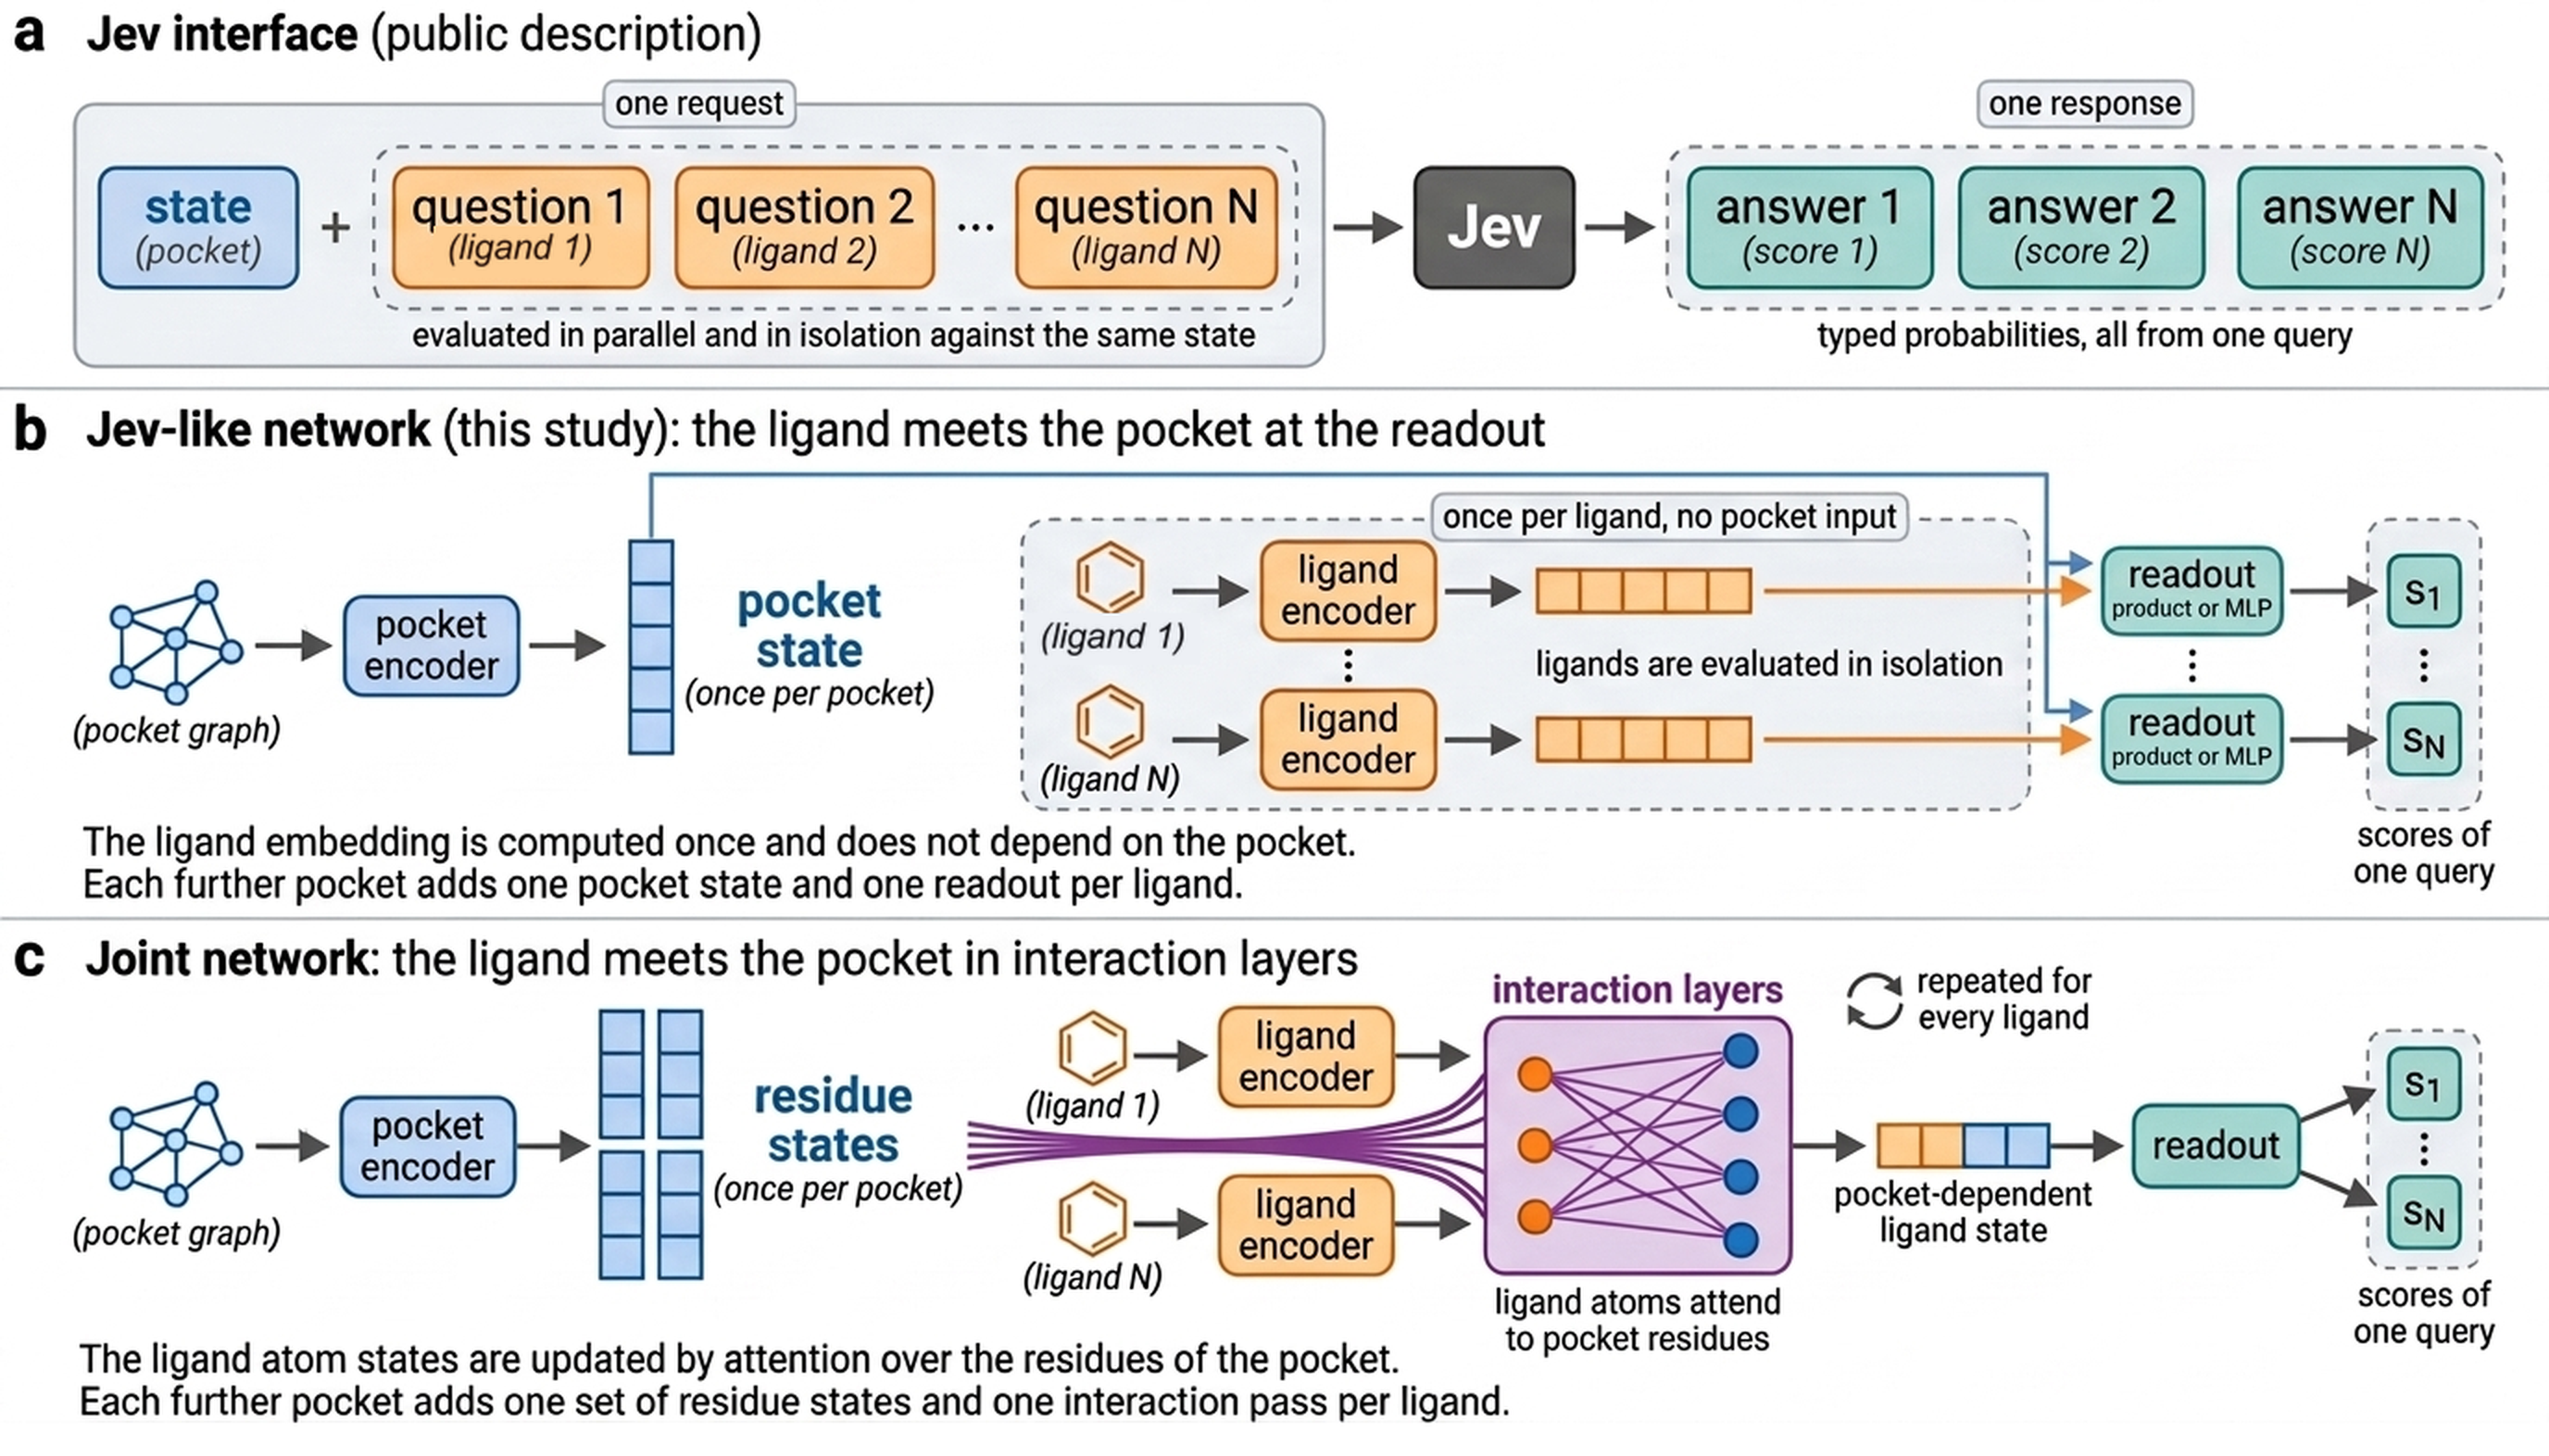
\includegraphics[width=\linewidth]{figures/fig1_concept}
\caption{The Jev interface and the two organizations of the surrogates. (a) Jev takes one state and several typed questions in one request, evaluates the questions in parallel and in isolation against the same state, and returns all answers in one response; the grey words in parentheses give the counterpart in this study. Blue marks the state, orange the questions and teal the answers, and the same colors mark the pocket, the ligands and the scores in b and c. (b) The Jev-like network encodes the pocket once into a cached state, embeds every ligand independently of the pocket and of the other ligands, and meets the pocket only at a cheap readout (a product of the pooled vectors for the dual encoder, a multilayer perceptron on the pooled vectors for the pooled network), so that each new pocket adds one pocket state and one readout per ligand. (c) In the joint cross-attention network the ligand atoms attend to the residues of the pocket in interaction layers, so that each new pocket adds one set of residue states and one interaction pass per ligand. The scores of all pairs rank the library for each pocket, and the best 10\% of the ranking are docked.}
\label{fig:concept}
\end{figure}
